% total_main.tex -- the eight section files inlined into one document, generated by
% scripts/flatten_paper.py.  Everything else (main.tex's preamble, style/, the .bib files, figure/) is
% unchanged and still required to build.  Edit the section files, not this one: regenerate it instead,
% or the next regeneration silently discards the edits.
%
\documentclass{article} % For LaTeX2e
% Target venue: ICLR 2027.  The kit under style/ is the 2025 one from the IGDM release; drop the
% 2027 .sty/.bst into style/ and change the two lines naming them.  Nothing else depends on the
% year.  Layout: this file + N_Section.tex are the manuscript, style/ is the venue kit, *.bib the
% bibliography, notes/ the prose companions that are NOT part of the build.
% 2026-09-05: the `times` option requests the ptm family, which has no TU (unicode) shapes under
% this engine, so every shape fell back to LM Roman regular and \textbf, \emph and \textsc were
% silently rendering as regular text -- paragraph headings and bold table rows included.  Forcing T1
% takes the legacy path, where ptm has its full set of shapes.
\usepackage[T1]{fontenc}
\usepackage{style/iclr2025_conference,times}

% Optional math commands from https://github.com/goodfeli/dlbook_notation.
\input{style/math_commands.tex}

\usepackage{hyperref}
\usepackage{url}

%%%%%%%%%%%%%%%%%%%%%%%%%%%%%% ADD PACKAGES %%%%%%%%%%%%%%%
\usepackage{subcaption}
\usepackage{amsmath}
\usepackage{amssymb}
\usepackage{amsthm}
\usepackage{cleveref}
\usepackage{booktabs}
\usepackage{multirow}
\usepackage{float}
\newcommand{\ie}{\emph{i.e.}}

\usepackage{algorithm}
\usepackage{algorithmic}

\usepackage{array}
% FLOAT PLACEMENT (2026-09-05).  Every table was declared [t] and there are seven in the experiments
% section alone, so LaTeX ran out of top slots, deferred them, and dumped the queue at the end of the
% document -- tab:ladder and tab:controls were landing on page 25 of a 13-page body.  Widening the
% float parameters gives the placement algorithm room, and placeins puts a barrier at each section so
% a float can no longer cross out of the section that declares it.
\usepackage[section]{placeins}
\setcounter{topnumber}{3}
\setcounter{bottomnumber}{2}
\setcounter{totalnumber}{4}
\renewcommand{\topfraction}{0.92}
\renewcommand{\bottomfraction}{0.6}
\renewcommand{\textfraction}{0.06}
\renewcommand{\floatpagefraction}{0.7}
\usepackage{sidecap}
\usepackage{xcolor}   % [table] dropped: another package loads xcolor first, and we use no row colours

\usepackage{textgreek}
\usepackage{tikz}
\usepackage{wrapfig}

\setlength{\aboverulesep}{0.6pt}
\setlength{\belowrulesep}{1.5pt}

% Propositions and proofs were running into the surrounding prose and were hard to find when
% skimming.  amsthm's plain style (bold header, italic body) plus a little air around the environment
% is enough; an earlier version drew a rule down the left margin, which read as a quote block.
\theoremstyle{plain}
\newtheorem{proposition}{Proposition}
\newtheorem{corollary}{Corollary}
\makeatletter
\def\thm@space@setup{%
  \thm@preskip=1.4\parskip \@plus 3pt \@minus 1pt
  \thm@postskip=\thm@preskip}
\makeatother

% Run-in headings carry the structure of the experiments section, so give them room to be seen.
\makeatletter
\renewcommand{\paragraph}{\@startsection{paragraph}{4}{\z@}%
  {1.8ex \@plus 0.7ex \@minus .2ex}{-0.7em}%
  {\normalfont\normalsize\bfseries}}
\makeatother
\newcommand{\dg}{\textsuperscript{\dag}}
\newcommand{\ddg}{\textsuperscript{\ddag}}
%%%%%%%%%%%%%%%%%%%%%%%%%%%%%%%%%%%%%%%%%%%%%%%%%%%%%%%%%%%%

% Title framing note: an earlier version ended "...without a Robust Teacher", which invites the
% reading "so with a robust teacher you lose" -- and we would, since IGDM+AdaAD reaches
% 64.44/30.32 on this architecture from a WRN-28-10 teacher.  That is a ranking claim against a
% line this paper does not compete with.  The register here follows B-MTARD and ARREST, whose
% titles both name the goal ("Mitigating the Accuracy-Robustness Trade-off") and the mechanism,
% and claim nothing about what is unnecessary.
\title{Clean Feature Anchoring: Mitigating the Accuracy--Robustness\\
Trade-off by Self-Distilling a Naturally Trained Model}

\author{
Anonymous authors\\
Paper under double-blind review
}

\newcommand{\fix}{\marginpar{FIX}}
\newcommand{\new}{\marginpar{NEW}}

% \iclrfinalcopy   % uncomment only for the camera-ready; submissions must stay anonymous

\begin{document}

\maketitle

%% ============================================================================
%% 0_Abstract.tex
%% ============================================================================

\begin{abstract}
Adversarial training improves robustness but often sacrifices accuracy on clean
data, leading to a persistent clean--robust trade-off. We address this trade-off
by first learning a high-accuracy clean self-teacher from natural images and then
preserving its clean knowledge while adversarially training the student. We
propose Clean Feature Anchoring (CFA), which trains the student to maintain the
teacher's clean representation under adversarial perturbations while retaining
the teacher's classifier.
We show that standard knowledge distillation approaches regression onto a fixed
clean target as the temperature increases, motivating the direct feature
anchoring used in CFA. We further show that keeping adversarial student features
close to this clean target simultaneously preserves their agreement with the
teacher on clean inputs and limits their variation within the perturbation
neighborhood. Our analysis also reveals that higher teacher clean accuracy does
not necessarily lead to better clean performance after robust training.
Finally, we observe that the same perturbation magnitude can affect the anchoring
objective differently across training samples. CFA therefore assigns smaller
perturbation radii to more sensitive samples and larger radii to less sensitive
ones while keeping the average perturbation budget fixed. Across CIFAR-10,
CIFAR-100, and Tiny-ImageNet, CFA achieves state-of-the-art clean--robust
trade-offs among the compared methods, retaining high clean accuracy while
maintaining strong adversarial robustness.
\end{abstract}

\section{Introduction}
\label{sec:intro}

Adversarial training is one of the most effective approaches to improving
robustness against adversarial perturbations, but this robustness often comes
at the cost of accuracy on clean data
\citep{PGD,tsipras2018robustness,TRADES}. This persistent clean--robust
trade-off raises a natural question: can a model acquire adversarial robustness
while retaining more of the knowledge that supports strong clean performance?

Several approaches seek to mitigate the clean--robust trade-off by leveraging
knowledge from naturally trained models. Such models provide accurate
predictions and representations on clean inputs, making them useful references
for preserving clean performance during adversarial training. Existing methods
incorporate this knowledge through teacher supervision or regularization.
However, clean knowledge can still be altered as the student adapts to
adversarial perturbations, leaving open how it can be preserved throughout
robust training.

We approach this problem by separating the learning of clean knowledge from
the subsequent learning of robustness. A clean self-teacher is first trained
on natural images and then fixed, providing a stable reference for the student
during adversarial training. Importantly, a more accurate clean teacher does
not necessarily transfer more clean performance to the robust student: we find
that teachers with similar clean accuracy can produce different transfer
outcomes, and that increasing teacher accuracy does not consistently improve
student clean accuracy. This motivates treating the teacher as a fixed source
of clean knowledge rather than assuming that its clean accuracy alone
determines the quality of robust transfer.

We instantiate this perspective with \textbf{Clean Feature Anchoring (CFA)}.
We first train a clean self-teacher on natural images and initialize the
student from this model. During adversarial training, CFA matches the student's
representation of an adversarial input to the self-teacher's fixed
representation of the corresponding clean input, while retaining the inherited
classifier. The teacher is therefore not required to provide robustness or
targets on adversarial inputs. Instead, it serves as a fixed clean reference:
the self-teacher defines what clean knowledge should be preserved, while
adversarial training determines the neighborhood over which the student learns
to preserve it.

\begin{figure}[t]
  \centering
  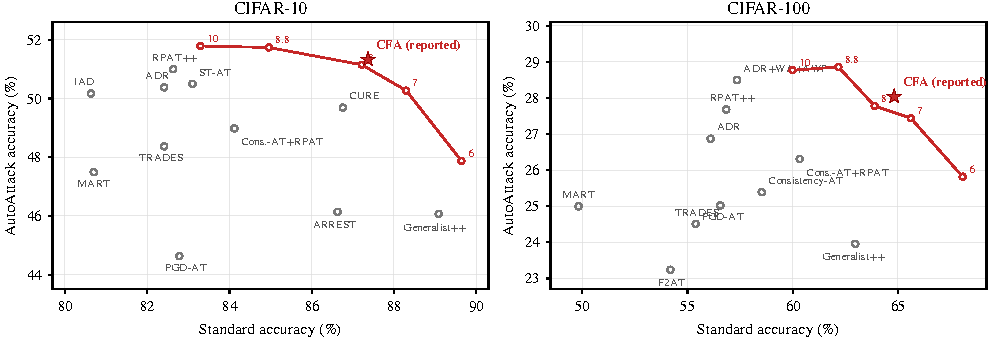
\includegraphics[width=\linewidth]{figure/frontier.pdf}
  \caption{Clean--AutoAttack trade-off on CIFAR-10 and CIFAR-100 with
  ResNet-18 at \(\epsilon=8/255\). Grey points are published results
  (\Cref{tab:published}); the CFA curve varies the training radius over
  100-epoch runs, and the star denotes the reported 150-epoch result trained
  at \(\epsilon_{\mathrm{train}}=8/255\).}
  \label{fig:frontier}
\end{figure}

CFA anchors the student's adversarial representations to a fixed clean
reference. We show that controlling this anchor simultaneously keeps the
student's clean representation close to the teacher and limits its variation
within the adversarial neighborhood.

The same perturbation magnitude, however, can affect the anchoring objective
differently across training samples. We therefore introduce
\emph{sensitivity-matched perturbation budgets}, assigning smaller
perturbation radii to more sensitive samples and larger radii to less
sensitive ones while preserving the average perturbation budget.

Across CIFAR-10, CIFAR-100, and Tiny-ImageNet, CFA achieves state-of-the-art
clean--robust trade-offs among the compared methods, consistently combining
high clean accuracy with strong adversarial robustness.

Our contributions are summarized as follows:
\begin{itemize}
  \item We introduce a clean self-teacher framework for mitigating the
  clean--robust trade-off by separating the learning of clean knowledge from
  the subsequent learning of robustness. CFA instantiates this principle by
  anchoring adversarial student representations to a fixed clean teacher
  representation.

  \item We analyze the role of the fixed clean anchor in adversarial training.
  We show that controlling the anchor simultaneously keeps the student's clean
  representation close to the teacher and limits its variation within the
  adversarial neighborhood. We further find that teacher clean accuracy alone
  does not determine how well clean performance is retained after adversarial
  training.

  \item We introduce sensitivity-matched perturbation budgets, which
  redistribute a fixed batch perturbation budget according to the local
  sensitivity of the anchoring objective, complementing the fixed clean target
  with example-dependent adversarial neighborhoods.
\end{itemize}

\section{Related Work}
\label{sec:related}

\paragraph{Adversarial training and its targets.}
PGD adversarial training optimizes a model on worst-case inputs \citep{PGD}; TRADES separates clean
prediction from local consistency \citep{TRADES}, and MART reweights misclassified examples
\citep{MART}. Subsequent work improves generalization through label smoothing, consistency
regularization, weight averaging, and adversarial weight perturbation
\citep{pang2020bag,tack2022consistency,robustoverfit,2020_awp}. ADR replaces one-hot labels with
targets produced by an annealed momentum teacher \citep{adr}. These approaches motivate our study
of how the supervisory target affects the clean--robust trade-off.

\paragraph{Predictive targets in adversarial distillation.}
ARD transfers a robust teacher's predictions during adversarial training \citep{ard}. RSLAD emphasizes
robust soft labels \citep{rslad}, IAD discounts unreliable teacher guidance \citep{iad}, and AdaAD uses
the teacher in both adversarial-example generation and student optimization \citep{adaad}. IGDM adds
the teacher's local input geometry to logit-based distillation \citep{igdm}. These methods are designed
to inherit robustness from an adversarially trained teacher. Our target instead comes from a natural
teacher at the clean input and remains fixed during the student's inner maximization.

\paragraph{Guidance from naturally trained models.}
BGAT is the closest direct-regression precedent: it matches adversarial logits to a fixed natural
teacher's clean logits, and LBGAT extends this to a jointly trained natural branch \citep{lbgat}.
Our logit control confirms that this fixed-clean-target principle is not specific to features. CFA
uses the full clean representation with an inherited fixed classifier, and our analysis focuses on
what a fixed clean anchor controls, how teacher properties relate to transferability, and how its
perturbation neighborhood is allocated. ARREST starts
from a naturally pretrained model and regularizes latent representations while retaining adversarial
cross-entropy and noisy replay \citep{arrest}. HAT uses a natural helper to label examples outside the
training ball \citep{hat}, and B-MTARD combines clean and robust teachers with adaptive temperature
and loss balancing \citep{bmtard}.

\paragraph{Sample-dependent perturbation budgets.}
IAAT and CAT adapt the training radius to sample difficulty, while MMA directly increases an
input-space margin \citep{iaat,cat,mma}. Our allocation has a different source: it redistributes a
fixed batch budget according to the input sensitivity of the loss being optimized. The comparison is
therefore not between adaptive and uniform radii alone, but between the signals used to assign the
same budget.

%% ============================================================================
%% 2_Analysis.tex
%% ============================================================================

\section{Analysis}
\label{sec:analysis}

Adversarial training often improves robustness at the cost of clean accuracy.
To mitigate this trade-off, we first learn a clean self-teacher from natural
images and then use it as a fixed reference while adversarially training the
student. A central question is how this clean knowledge can be preserved under
adversarial perturbations.

We begin with standard knowledge distillation, which matches
temperature-scaled teacher and student output distributions through KL
divergence, and examine its high-temperature behavior. We then study the
fixed clean target used by CFA and characterize what controlling this anchor
implies for the student's representation. Finally, we examine how teacher
clean accuracy relates to the clean performance retained by the adversarially
trained student.

\subsection{From Knowledge Distillation to a Fixed Clean Target}
\label{sec:fragile}

Let \(f=h\circ\Phi\), where \(\Phi\) is a feature map and
\(h(z)=Wz+b\) is a linear classifier producing logits
\(f(x)\in\mathbb{R}^{C}\) for \(C\) classes. Subscripts \(t\) and \(s\)
denote the frozen clean self-teacher and student, respectively. For a clean
input \(x\) and a perturbed input \(x'\in B(x,\epsilon)\), standard knowledge
distillation with a shared temperature \(\tau\) matches the teacher and student
output distributions
\begin{equation}
q_t^\tau(x)
=
\operatorname{softmax}\!\left(f_t(x)/\tau\right),
\qquad
p_s^\tau(x')
=
\operatorname{softmax}\!\left(f_s(x')/\tau\right)
\end{equation}
by minimizing
\(\tau^2 D_{\rm KL}(q_t^\tau(x)\|p_s^\tau(x'))\).

As \(\tau\) increases, the output distributions become softer. After the usual
\(\tau^2\) scaling, however, the distillation objective retains information
about the relative structure of the underlying logits. Let
\(\mathbf{1}\in\mathbb{R}^{C}\) denote the all-ones vector and define the
centered logits
\[
\bar f
=
f-\frac{1}{C}\mathbf{1}\mathbf{1}^{\top}f,
\]
which subtract the mean logit from every coordinate. For fixed teacher and
student logits,
\begin{equation}
\lim_{\tau\to\infty}
\tau^2 D_{\rm KL}(q_t^\tau(x)\|p_s^\tau(x'))
=
\frac{1}{2C}
\left\|
\bar f_t(x)-\bar f_s(x')
\right\|_2^2.
\label{eqn:kd_limit}
\end{equation}
The centering reflects the invariance of softmax to adding the same constant
to every logit. Thus, in the high-temperature limit, standard knowledge
distillation approaches direct matching between the student's perturbed output
and a fixed clean teacher target, up to this shift invariance.

This establishes a connection between distribution matching and direct
matching to a fixed clean target. CFA applies this fixed-target formulation
to intermediate representations:

\begin{equation}
\mathcal L_{\rm anchor}(x)
=
\max_{x'\in B(x,\epsilon)}
\left\|
\Phi_s(x')-\Phi_t(x)
\right\|_2^2.
\label{eqn:anchor_percell}
\end{equation}
Here, the clean teacher feature \(\Phi_t(x)\) serves as a fixed target, and
CFA trains the student to preserve this representation under perturbations
within \(B(x,\epsilon)\).

\begin{figure}[t]
  \centering
  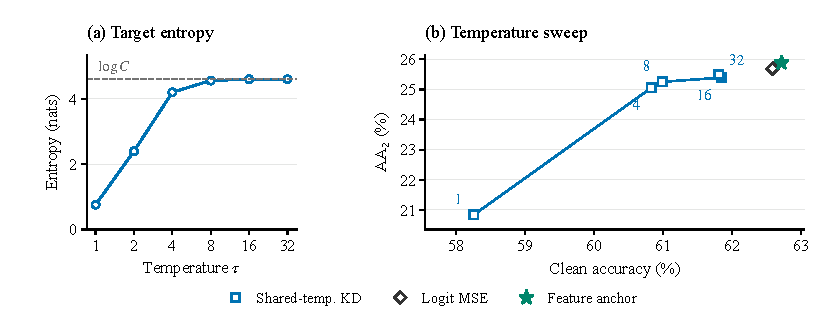
\includegraphics[width=\linewidth]{figure/analysis_targets.pdf}
  \caption{Target comparison on CIFAR-100 (ResNet-18).
  (a) Entropy of the clean teacher target as the shared temperature increases.
  (b) Clean accuracy and AutoAttack (AA) under shared-temperature knowledge
  distillation (KD), direct logit regression, and feature regression.
  Exact values are provided in \Cref{tab:targetcomparison_values}.}
  \label{fig:targetcomparison}
\end{figure}

Figure~\ref{fig:targetcomparison} shows the corresponding empirical trend:
as the temperature increases, KD approaches the operating point of direct
regression, consistent with \Cref{eqn:kd_limit}. CFA uses the feature
representation as its clean anchor and achieves a favorable clean--robust
operating point. We next examine what controlling this anchor implies for
the student.

\subsection{What the Anchor Controls}
\label{sec:decomp}

The fixed clean anchor provides a single reference for the student's
representations throughout the adversarial neighborhood. We now ask what is
controlled when the worst-case discrepancy from this reference is kept small.
For \(B=B(x,\epsilon)\), define
\begin{equation}
L=\max_{x'\in B}\|\Phi_s(x')-\Phi_t(x)\|_2,\quad
F=\|\Phi_s(x)-\Phi_t(x)\|_2,\quad
O=\max_{x',x''\in B}\|\Phi_s(x')-\Phi_s(x'')\|_2.
\label{eqn:LFO}
\end{equation}
Here, \(F\) measures the student's discrepancy from the teacher on the clean
input, while \(O\) measures the variation of the student's representation
within the adversarial neighborhood.

\begin{proposition}[Fixed-anchor decomposition]\label{prop:decomp}
For every \(x\) and \(\epsilon\ge0\),
\begin{equation}
L\le F+O\le3L.
\label{eqn:decomp}
\end{equation}
\end{proposition}

The result follows directly from the triangle inequality. Since
\(x\in B(x,\epsilon)\), we have \(F\le L\). Moreover, for any
\(x',x''\in B(x,\epsilon)\),
\begin{equation}
\|\Phi_s(x')-\Phi_s(x'')\|_2
\le
\|\Phi_s(x')-\Phi_t(x)\|_2
+
\|\Phi_s(x'')-\Phi_t(x)\|_2
\le 2L,
\end{equation}
so \(O\le2L\). Conversely, inserting \(\Phi_s(x)\) between
\(\Phi_s(x')\) and \(\Phi_t(x)\) gives \(L\le F+O\), completing the
bound. The full proof and discussion are provided in
\Cref{app:anchor_scope}.

Thus, keeping the worst-case anchor discrepancy small simultaneously keeps
the clean student representation close to the teacher and limits its variation
within the perturbation region. Notably, this conclusion depends only on the
teacher representation at the clean input; the teacher itself need not be
robust throughout the neighborhood.


\subsection{Does Better Clean Teacher Performance Transfer to the Student?}
\label{sec:teacher_transfer}

The fixed clean anchor raises a natural question: does a better clean teacher
necessarily provide a better target for the adversarially trained student?

\begin{figure}[H]
  \centering
  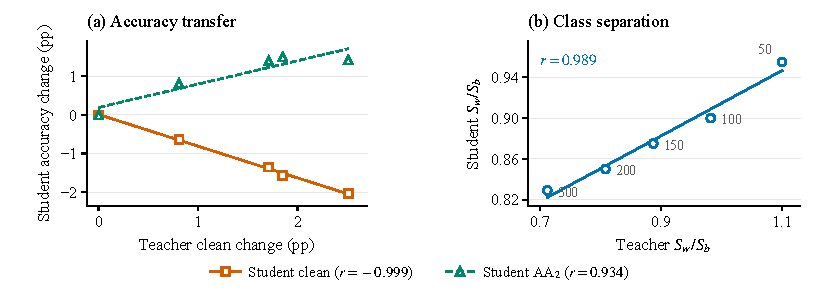
\includegraphics[width=0.92\linewidth]{figure/teacher_checkpoint_trends.pdf}
  \caption{
  Transfer from clean self-teachers at different stages of training on
  CIFAR-100 (ResNet-18).
  (a) Changes in teacher clean accuracy and resulting student clean accuracy
  and AA relative to the 50-epoch teacher.
  (b) Ratio of within-class scatter \(S_w\) to between-class scatter \(S_b\)
  for teacher and student features. \(S_w\) measures the dispersion of features
  around their corresponding class centroids, whereas \(S_b\) measures the
  separation among class centroids; lower \(S_w/S_b\) indicates more compact
  within-class features relative to between-class separation. Labels denote
  teacher epochs, and lines are least-squares fits. Exact values are reported in
  \Cref{tab:teacherladder_values}.
  }
  \label{fig:teacherladder}
\end{figure}

As the clean teacher improves along its training trajectory, the resulting
student does not exhibit a corresponding improvement in clean accuracy
(\Cref{fig:teacherladder}). Instead, different teacher checkpoints lead to
different clean--robust operating points. The same overall trend appears for
an independently trained teacher trajectory
(\Cref{tab:teacherladder_seed1}).

We also examine the within-to-between scatter ratio \(S_w/S_b\) on
unit-normalized clean features. Its evolution across teacher checkpoints is
reflected in the resulting students, indicating that the transferred
representation changes even when teacher quality is summarized only by clean
accuracy. We treat this association as descriptive rather than causal.

A complementary comparison uses two self-teachers with nearly identical
clean accuracy but different training schemes. Despite their similar clean
performance, they produce substantially different student clean accuracies
while yielding similar robustness (\Cref{tab:matchedteacher}). Together,
these results show that teacher clean accuracy alone is an incomplete
descriptor of transferability. We therefore use the 200-epoch checkpoint as
a fixed reference teacher in the remaining experiments.

\begin{table}[!htbp]
  \centering
  \small
  \setlength{\tabcolsep}{4.5pt}
  \caption{Transfer from accuracy-matched clean self-teachers on CIFAR-100
  (ResNet-18; 50-epoch students). Feature sensitivity is measured on held-out
  data.}
  \label{tab:matchedteacher}
  \begin{tabular}{lrrcrr}
    \toprule
    & \multicolumn{2}{c}{Teacher} && \multicolumn{2}{c}{Student} \\
    \cmidrule(lr){2-3}\cmidrule(lr){5-6}
    Natural training & Clean & Sensitivity && Clean & AA \\
    \midrule
    Label smoothing \(0.1\) & 78.76 & 3.16 && 59.62 & 25.72 \\
    Mixup & 78.62 & 4.82 && 63.80 & 25.70 \\
    \bottomrule
  \end{tabular}
\end{table}

\subsection{Sensitivity to Input Perturbations}
\label{sec:sensitivity_analysis}

The fixed clean target specifies what should be preserved, but the same
input-space perturbation radius need not have the same effect on the anchoring
objective for every training sample. For
\[
\ell_{\rm anc}(x';x_i)
=
\|\Phi_s(x')-\Phi_t(x_i)\|_2^2,
\]
the first-order change under an \(\ell_\infty\) perturbation of radius \(e\)
satisfies
\begin{equation}
\max_{\|\delta\|_\infty\le e}
\left\langle
\nabla_{x'}\ell_{\rm anc},\delta
\right\rangle
=
e\|\nabla_{x'}\ell_{\rm anc}\|_1.
\label{eqn:firstorder}
\end{equation}
Thus, a common perturbation radius can induce different changes in the
anchoring objective across training samples when their local sensitivities
differ. This motivates adapting the perturbation radius to each sample's
sensitivity.

\section{Method}
\label{sec:method}

The preceding analysis motivates two components of CFA: a fixed clean
representation provides the target to preserve, while local sensitivity
guides the perturbation radius assigned to each training sample.

\subsection{Clean Feature Anchoring}
\label{sec:anchor}

Let \(\Phi_t,h_t\) denote the frozen clean self-teacher. The student is
initialized from the teacher, \(\Phi_s\leftarrow\Phi_t\) and \(h_s=h_t\),
after which only \(\Phi_s\) is optimized. For each clean example,
\begin{equation}
x_{\rm adv}
=
\arg\max_{x'\in B(x,\epsilon)}
\|\Phi_s(x')-\Phi_t(x)\|_2^2,
\qquad
\mathcal L_{\rm CFA}
=
\mathbb E_x
\|\Phi_s(x_{\rm adv})-\Phi_t(x)\|_2^2.
\label{eqn:anchor}
\end{equation}
We approximate the inner maximization with randomly initialized PGD. Inference
uses the inherited classifier \(h_t\circ\Phi_s\). The full procedure is given
in \Cref{alg:cfa}.

\subsection{Sensitivity-Matched \(\epsilon\)}
\label{sec:angeps}

Motivated by the sensitivity analysis in
\Cref{sec:sensitivity_analysis}, we adapt the perturbation radius to each
training sample. More sensitive samples receive smaller radii, whereas less
sensitive samples receive larger radii. Given a local sensitivity score
\(g_i>0\) for sample \(i\), we set
\begin{equation}
\epsilon_i
=
N\epsilon
\frac{g_i^{-p}}{\sum_{j=1}^{N} g_j^{-p}},
\label{eqn:angeps_ideal}
\end{equation}
where \(N\) is the batch size, \(\epsilon\) is the target mean radius, and
\(p\) controls the strength of sensitivity matching. When \(p=0\), all
samples receive the same radius \(\epsilon\); for \(p>0\), the radius decreases
with sensitivity. The normalization ensures
\(\frac{1}{N}\sum_{i=1}^{N}\epsilon_i=\epsilon\), so the average perturbation
budget is unchanged.

For \(p=1\), the unnormalized rule satisfies
\(\epsilon_i g_i \propto 1\), approximately balancing the first-order
perturbation effect across training samples. This relation motivates the
allocation rule but does not imply exact equalization of the nonlinear
anchoring loss.

We evaluate the effect of sensitivity matching and the importance of assigning
the resulting radii to their corresponding samples in
\Cref{tab:finalallocation,tab:allocation}. Details on sensitivity estimation,
radius clipping, and sensitivity-norm choices are provided in
\Cref{app:box}.

\section{Experiments}
\label{sec:exp}

\subsection{Experimental Settings}

We evaluate CFA on CIFAR-10, CIFAR-100
\citep{krizhevsky2009learning}, and Tiny-ImageNet-200
\citep{le2015tiny}. We use ResNet-18 as the default architecture and
additionally report results with WideResNet-34-10. Unless stated otherwise,
the clean self-teacher is trained on natural images for 200 epochs and then
frozen. The student is initialized from the teacher, with the inherited
classifier kept fixed during adversarial training.

The main CIFAR experiments use 150 training epochs, AdamW with a one-cycle
learning-rate schedule, 10-step projected gradient descent (PGD-10),
\(\epsilon_{\rm train}=8/255\), sensitivity-matched perturbation radii with
\(p=1\), weight averaging (WA), and adversarial weight perturbation (AWP).

For comparison, we include standard adversarial training baselines
(PGD-AT, TRADES, and MART), adversarial distillation methods
(ARD, RSLAD, AdaAD, and AdaAD+IGDM), and methods that are particularly
relevant to CFA's clean--robust setting. The latter include LBGAT and
ARREST, which use natural teachers; HAT and RPAT++, which target the
clean--robust trade-off; and ADR, which uses self-distillation. We use
the respective training recipes of each baseline, with the same natural
teacher as CFA for distillation methods where applicable.

We report clean accuracy and AutoAttack (AA) accuracy on the full test set
at \(\epsilon=8/255\), together with their arithmetic mean (Avg) and
harmonic mean (NRR). Dataset-specific settings, teacher statistics, attack
diagnostics, and additional controls are provided in
\Cref{app:repro,app:gradmask}.


\subsection{Main Results}

\begin{table}[!htbp]
  \centering
  \footnotesize
  \setlength{\tabcolsep}{3.2pt}
  \caption{
  ResNet-18 results under \(\ell_\infty\) perturbations with
  \(\epsilon=8/255\). All values are measured in our framework.
  \emph{T.} denotes the teacher assumed by each method: none (--),
  a natural model (nat.), or the method's own weight average (self).
  The CIFAR-100 CFA row reports the mean of three student seeds;
  all other rows are individual runs.
  }
  \label{tab:main}
  \begin{tabular}{llrrrrrrrr}
    \toprule
    & & \multicolumn{4}{c}{CIFAR-10}
      & \multicolumn{4}{c}{CIFAR-100} \\
    \cmidrule(lr){3-6}\cmidrule(lr){7-10}
    Method & T. & Clean & AA & Avg & NRR
           & Clean & AA & Avg & NRR \\
    \midrule
    PGD-AT & -- & 84.54 & 43.57 & 64.06 & 57.50
                 & 57.36 & 20.34 & 38.85 & 30.03 \\
    TRADES & -- & 81.71 & 49.16 & 65.44 & 61.39
                 & 55.28 & 23.55 & 39.42 & 33.03 \\
    MART   & -- & 80.41 & 45.56 & 62.99 & 58.16
                 & 53.86 & 22.72 & 38.29 & 31.96 \\
    \midrule
    ARD & nat. & 84.58 & 43.75 & 64.16 & 57.67
               & 57.61 & 20.24 & 38.93 & 29.96 \\
    RSLAD & nat. & 85.15 & 42.91 & 64.03 & 57.06
                 & 59.68 & 21.30 & 40.49 & 31.40 \\
    AdaAD & nat. & 85.39 & 46.22 & 65.81 & 59.98
                 & 59.79 & 23.19 & 41.49 & 33.42 \\
    AdaAD + IGDM & nat. & 85.01 & 45.50 & 65.26 & 59.27
                        & 48.25 & 19.48 & 33.87 & 27.75 \\
    LBGAT & nat. & -- & -- & -- & --
                 & 56.46 & 26.02 & 41.24 & 35.62 \\
    ARREST & nat. & 85.06 & 46.42 & 65.74 & 60.06
                  & \textbf{66.97} & 22.78 & 44.88 & 34.00 \\
    \midrule
    HAT & nat. & 84.59 & 48.81 & 66.70 & 61.90
               & 60.67 & 24.45 & 42.56 & 34.85 \\
    ADR & self & 83.36 & 49.72 & 66.54 & 62.29
               & 59.93 & 27.20 & 43.57 & 37.42 \\
    RPAT++ & -- & 82.41 & 50.75 & 66.58 & 62.82
                  & 55.93 & 27.36 & 41.64 & 36.74 \\
    \midrule
    \textbf{CFA (ours)}
      & nat.
      & \textbf{87.37} & \textbf{51.33}
      & \textbf{69.35} & \textbf{64.67}
      & \textbf{64.82} & \textbf{28.04}
      & \textbf{46.43} & \textbf{39.15} \\
    \bottomrule
  \end{tabular}
\end{table}

On CIFAR-100, CFA achieves \(64.82\%\) clean accuracy and \(28.04\%\)
AA, with an NRR of \(39.15\). Compared with ADR, the closest baseline
in NRR, CFA improves clean accuracy by \(4.89\) points, AA by \(0.84\)
points, and NRR by \(1.73\) points. On CIFAR-10, CFA achieves
\(87.37\%\) clean accuracy and \(51.33\%\) AA, with an NRR of
\(64.67\), \(1.85\) points above the closest baseline
(\Cref{tab:main}).

We additionally evaluate CFA on Tiny-ImageNet-200 and with
WideResNet-34-10 to examine whether the results persist beyond the
default CIFAR/ResNet-18 setting.

\begin{table}[!htbp]
  \centering
  \footnotesize
  \setlength{\tabcolsep}{3.2pt}
  \caption{
  Results on Tiny-ImageNet-200 with ResNet-18 and CIFAR-10 with
  WideResNet-34-10, measured in our framework.
  }
  \label{tab:scale}
  \begin{tabular}{llrrrrrrrr}
    \toprule
    & & \multicolumn{4}{c}{Tiny-ImageNet, ResNet-18}
      & \multicolumn{4}{c}{CIFAR-10, WRN-34-10} \\
    \cmidrule(lr){3-6}\cmidrule(lr){7-10}
    Method & T. & Clean & AA & Avg & NRR
           & Clean & AA & Avg & NRR \\
    \midrule
    PGD-AT & -- & 49.72 & 14.45 & 32.09 & 22.39
                 & 86.00 & 45.71 & 65.86 & 59.69 \\
    TRADES & -- & 46.98 & 15.95 & 31.46 & 23.83
                 & 85.13 & 48.99 & 67.06 & 62.19 \\
    MART & -- & 46.01 & 16.90 & 31.46 & 24.73
               & 85.29 & 47.06 & 66.18 & 60.65 \\
    \midrule
    ARD & nat. & 49.74 & 14.48 & 32.11 & 22.43
               & 86.35 & 45.52 & 65.94 & 59.61 \\
    RSLAD & nat. & 51.26 & 17.02 & 34.14 & 25.56
                 & 86.41 & 45.80 & 66.10 & 59.87 \\
    AdaAD & nat. & 51.59 & 16.79 & 34.19 & 25.33
                 & 86.80 & 46.84 & 66.82 & 60.85 \\
    LBGAT & nat. & 51.04 & 18.47 & 34.75 & 27.13
                 & 81.56 & 51.79 & 66.68 & 63.35 \\
    ARREST & nat. & \textbf{59.38} & 16.06 & 37.72 & 25.28
                  & 87.54 & 48.83 & 68.19 & 62.69 \\
    HAT & nat. & 52.57 & 17.28 & 34.93 & 26.01
               & 87.15 & 53.21 & 70.18 & 66.07 \\
    ADR & self & 47.66 & \textbf{20.85} & 34.25 & 29.01
               & 88.64 & 52.34 & 70.49 & 65.82 \\
    \midrule
    \textbf{CFA (ours)}
      & nat.
      & 55.16 & 20.54 & \textbf{37.85} & \textbf{29.93}
      & \textbf{88.67} & \textbf{55.29}
      & \textbf{71.98} & \textbf{68.11} \\
    \bottomrule
  \end{tabular}
\end{table}

On Tiny-ImageNet-200 with ResNet-18, CFA achieves \(55.16\%\) clean
accuracy and \(20.54\%\) AA, yielding an NRR of \(29.93\). With
WideResNet-34-10 on CIFAR-10, CFA achieves \(88.67\%\) clean accuracy
and \(55.29\%\) AA, with an NRR of \(68.11\)
(\Cref{tab:scale}). On CIFAR-100 with the same architecture, CFA obtains
\(65.04/30.14\) clean/AA, compared with \(64.50/29.04\) for ADR
(\Cref{tab:wrn100}).


\subsection{Ablation and Component Analysis}
\label{sec:components}
\paragraph{Clean feature anchoring.}

We first isolate the effect of the anchor objective by removing sensitivity
matching, weight averaging, and AWP. Under the same training recipe, CFA
improves both clean accuracy and AA over label-based adversarial training
(\Cref{tab:controls}). The advantage remains when the cross-entropy baseline
uses its own optimizer and training schedule.

We further compare the resulting feature geometry. We measure the
within-to-between class scatter ratio \(S_w/S_b\), the mean angle of each
feature to its own class centroid (\emph{Own}), and the mean angle from each
class centroid to its nearest other-class centroid (\emph{Gap}).

\begin{table}[t]
  \centering
  \small
  \setlength{\tabcolsep}{4pt}
  \caption{
  Feature geometry of CFA and label-based adversarial training on CIFAR-100.
  \emph{Own} is the mean sample-to-own-centroid angle, and \emph{Gap} is the
  mean angle from each class centroid to its nearest other-class centroid.
  Lower \(S_w/S_b\) and \emph{Own} indicate tighter within-class
  concentration, whereas larger \emph{Gap} indicates greater separation
  between class centroids. Angles are measured on unit-normalized features.
  }
  \label{tab:anchorgeometry}
  \begin{tabular}{lrrrcrrr}
    \toprule
    & \multicolumn{3}{c}{Clean}
    && \multicolumn{3}{c}{Adversarial} \\
    \cmidrule(lr){2-4}\cmidrule(lr){6-8}
    & \(S_w/S_b\) & Own & Gap
    && \(S_w/S_b\) & Own & Gap \\
    \midrule
    CFA
      & \textbf{0.709} & \textbf{26.3\(^{\circ}\)} & 29.2\(^{\circ}\)
      && \textbf{1.969} & \textbf{33.5\(^{\circ}\)} & 19.2\(^{\circ}\) \\
    Label CE
      & 3.744 & 52.2\(^{\circ}\) & \textbf{33.5\(^{\circ}\)}
      && 5.611 & 55.0\(^{\circ}\) & \textbf{28.2\(^{\circ}\)} \\
    \bottomrule
  \end{tabular}
\end{table}

As shown in \Cref{tab:anchorgeometry}, CFA produces substantially tighter
within-class feature concentration on both clean and adversarial inputs,
while the centroid gaps are not larger than those of the label-trained model.
The difference is therefore characterized primarily by within-class
concentration rather than increased separation between classes.

As an additional control, we apply teacher initialization, weight averaging,
and AWP to the baseline methods. Although these additions improve most
baselines, none reaches CFA's NRR (\Cref{tab:baselinestack}).


\paragraph{Sensitivity-matched radius allocation.}
The allocation rule is motivated by the hypothesis that a common input-space
radius does not correspond to a common perturbation effect under the anchor
loss. We test this in two steps. We first compare sensitivity matching with a
uniform radius while holding the teacher, training schedule, mean radius, WA,
and AWP fixed. We then ask whether the sensitivity signal itself matters or
whether heterogeneous radii alone are sufficient.
\begin{table}[!htbp]
  \centering
  \small
  \setlength{\tabcolsep}{5pt}
  \caption{
  Clean-target regression in the final CIFAR-100 recipe
  (ResNet-18, 150 epochs, \(\epsilon_{\mathrm{train}}=8/255\)).
  Feature rows report mean \(\pm\) sample standard deviation over three
  student seeds and differ only in \(p\); logit regression is one run at
  \(p=1\).
  }
  \label{tab:finalallocation}
  \begin{tabular}{lrrr}
    \toprule
    Target and radius & Clean & AA & NRR \\
    \midrule
    Features, uniform (\(p=0\))
      & \(62.63\pm0.22\)
      & \(28.01\pm0.20\)
      & \(38.71\pm0.21\) \\
    Features, sensitivity-matched (\(p=1\))
      & \(\mathbf{64.82\pm0.07}\)
      & \(\mathbf{28.04\pm0.09}\)
      & \(\mathbf{39.15\pm0.09}\) \\
    Logits, sensitivity-matched (\(p=1\))
      & 64.49 & 27.85 & 38.90 \\
    \bottomrule
  \end{tabular}
\end{table}

Across three paired runs, sensitivity matching improves clean accuracy by
\(2.19\pm0.20\) points while AA changes by only \(0.03\pm0.23\) points. The
clean gain appears in every seed, whereas the AA difference is within
run-to-run variation. Direct logit regression remains close to feature
regression, consistent with the fixed-target interpretation.

\paragraph{Does the allocation signal matter?}
\begin{table}[!htbp]
  \centering
  \small
  \setlength{\tabcolsep}{4.5pt}
  \caption{
  Radius-allocation signals under the same mean radius on CIFAR-100 with
  ResNet-18, trained for 100 epochs with WA and AWP.
  \(\mathrm{sd}(w)\) measures multiplier dispersion.
  }
  \label{tab:allocation}
  \begin{tabular}{lrrrr}
    \toprule
    Allocation & \(\mathrm{sd}(w)\) & Clean & AA & NRR \\
    \midrule
    Uniform
      & 0 & 60.42 & 28.42 & 38.66 \\
    Sensitivity
      & 0.32 & \textbf{62.17} & \textbf{28.86} & \textbf{39.42} \\
    Same multipliers, difficulty order
      & 0.32 & 60.90 & 28.06 & 38.42 \\
    Difficulty magnitude
      & 0.39 & 61.27 & 28.12 & 38.55 \\
    Logit margin
      & 0.42 & 61.07 & 27.79 & 38.20 \\
    \bottomrule
  \end{tabular}
\end{table}

The ``same multipliers, difficulty order'' control is especially informative:
it preserves the sensitivity-derived set of radii and changes only which
examples receive them. This reassignment reduces AA by \(0.80\) points and
NRR by \(1.00\) point. Thus the observed benefit cannot be attributed to
radius heterogeneity alone; the correspondence between local sensitivity and
the assigned neighborhood contributes to the result. Additional recipe,
radius, and WA/AWP controls are reported
in \Cref{tab:baselinestack,tab:radius,tab:stackboth,tab:ladder}.

\section{Conclusion}
We introduced CFA as a way to mitigate the clean--robust trade-off by
separating the learning of clean knowledge from the learning of robustness. A
naturally trained self-teacher first provides a high-accuracy clean reference;
the student then learns robustness while matching that fixed reference over
its adversarial neighborhood. Our analysis connects this view to fixed
clean-target regression, characterizes the joint fidelity and local-variation
control induced by the anchor, and shows that teacher clean accuracy alone
does not determine robust transfer. Sensitivity-matched radii complement the
anchor by redistributing a fixed perturbation budget according to the local
response of the training objective. Across datasets, architectures, and
controls, the results support clean self-teaching as a practical route to
retaining clean performance during adversarial training without requiring an
adversarial teacher or a label objective in the robust stage. The results also
delineate the scope of this mechanism: fixed-target anchoring does not imply
that feature coordinates are intrinsically preferable to logits, and clean
teacher accuracy alone does not identify the most transferable teacher.
Understanding which properties of a clean representation govern its
transferability under adversarial training remains an open direction.

% The appendix is kept in a separate file so the nine-page main body can be
% edited independently while preserving cross-references in the full build.
\clearpage
\input{appendix_revised_v6.tex}

\bibliography{AT,cfa}
\bibliographystyle{style/iclr2025_conference}
\end{document}
